\documentclass[letterpaper, 10pt]{article}
\usepackage{tikz}
\usepackage[utf8]{inputenc}
\usepackage[T1]{fontenc}
\usepackage[french]{babel}
\usepackage{geometry}
\usepackage{titling}
\usepackage{graphicx}
\usepackage{listings}
\usepackage{color}
\usepackage{url}
\usepackage{enumitem}

\geometry{a4paper, margin=1in}

\title{IFT3913 - Qualité de Logiciel et Métriques \\ TP 4}
\author{Yalin Mo (20199655) \\ Vennila Sooben (20235256)}
\date{\today}

\begin{document}
\maketitle

\section*{Objectif}
Dans le cadre de ce TP, l'objectif était de tester le logiciel "Currency Converter". Le code est accessible via le dépôt Git à \url{https://github.com/mfamelis/currency-converter-in-java}. Nous avons focalisé nos tests sur deux méthodes du "Currency Converter":
\begin{itemize}
    \item \texttt{currencyConverter.MainWindow.convert(String, String, ArrayList<Currency>, Double)}
    \item \texttt{currencyConverter.Currency.convert(Double, Double)}
\end{itemize}

\section*{\textsc{1. Tests Boîte Noire}}
\item \textbf{Choix des cas de tests}
Nous avons choisi les cas de tests en nous basant sur les classes d'équivalence et l'analyse des valeurs frontières, couvrant ainsi un large éventail de scénarios possibles. Nous avons également pris en compte les spécifications du "Currency Converter" lors de la création de nos tests.


\subsection*{Méthode \texttt{currencyConverter.MainWindow.convert}}
Nous avons suivi une approche de partitionnement du domaine en classes d'équivalence et d'analyse des valeurs frontières pour les devises et les montants. En effet, les valeurs normales, extremes et invalides ont été utilisées.


\begin{itemize} 
    \item \textbf{Analyse des valeurs frontières pour les montants :}
    \begin{enumerate}
        \item Montant normale : Valide
        \begin{itemize}
            \item 10
        \end{itemize}
        \item Montants extrêmes valides : Valide
        \begin{itemize}
            \item 0
            \item 1000000
        \end{itemize}
         \item Montants proches des limites : Exception
         \begin{itemize}
            \item -0.01
            \item 1000000.01
        \end{itemize}
        \item Montant négatif : Exception
        \begin{itemize}
            \item -1
        \end{itemize}
     \end{enumerate}
     \item \textbf{Analyse des valeurs frontières pour les monnaies :}
    \begin{enumerate}
        \item Monnaie normale : Valide
        \begin{itemize}
            \item USD, CAD, GBP, EUR, CHF, AUD.
        \end{itemize}
        \item Monnaie non-inclue dans l'ArrayList : Exception
        \begin{itemize}
            \item USD, CAD, GBP, EUR, CHF, AUD. dans l'ArrayList mais test avec XYZ
        \end{itemize}
     \end{enumerate}
    \item \textbf{Hypothèses pour les entrées non-valides :}
        \begin{itemize}
            \item Pour les devises invalides, nous nous attendons à un message d'erreur ou à l'ignorance de la conversion.
            \item Pour les montants invalides, nous anticipons une exception ou un message d'erreur.\\
        \end{itemize}

\item \textbf{Problématique Identifiée}

Au cours des tests, il a été observé que l'application présente un comportement inattendu dans certaines situations. Cependant, en tant que testeur boîte noire, nous ne sommes pas en mesure de fournir des détails sur l'implémentation interne, mais plutôt de signaler les comportements observés.
\\
\item \textbf{Recommandations}

\begin{itemize}
    \item Il faut une vérification approfondie de la fonctionnalité de conversion de devises.
    \item Il faut poursuivre avec des tests boîtes blanche\\
\end{itemize}
\item \textbf{Conclusion}\\
La spécification aurait dû fournir plus de détails notamment sur le ArrayList<Currency> et sur la classe Currency. En effet, un travail supplémentaire était nécessaire. Ceci ne respecte pas les tests boites noirs mais afin de mener à bien l'écriture de test, nous avons utilises les getters disponibles. Ceci était dans le but de rester dans l'esprit de ne pas regarder le code de MainWindow.convert. La seule impasse que nous nous sommes accordés était de vérifier quelle méthode utiliser pour initialiser l'ArrayList<Currency>. \\De plus, les tests ne passent pas. En effet, non seulement CAD et AUD était indisponible mais en plus nous obtenons des 0 constamment. 
\end{itemize}
\subsection*{Méthode \texttt{currencyConverter.Currency.convert}}
Nous avons suivi une approche de partitionnement du domaine en classes d'équivalence et d'analyse des valeurs frontières pour les devises et les montants.

\begin{itemize}
    \item \textbf{Classes d'équivalence pour les devises :}
        \begin{enumerate}
          \item Nous utilisons plusieurs devises pour représenter différentes classes d'équivalence. Chaque devise représente une classe d'équivalence distincte, comme le US Dollar (USD), Euro (EUR),  British Pound(GBP), etc. Nous nous assurons que nos tests couvrent ces différentes devises pour vérifier si la méthode currency.convert fonctionne correctement lorsqu'elle traite des conversions entre différentes devises.
        \end{enumerate}
    \item \textbf{Classes d'équivalence pour les montants :}
        \begin{enumerate}
            \item Dans nos tests, nous prenons en compte les classes d'équivalence suivantes :
            \begin{itemize}
            
            \item Montant positif —— 500000.00 : nous testons les montants positifs pour nous assurer que la méthode calcule correctement les conversions avec des montants positifs.
            
            \item Montant plus que la limite ——1000000.01: le programme va lancer une exception car le montant maximum disponible est 1000000
            
            \item  Montant négatif —— -1.00 : nous testons les montants négatifs pour nous assurer que la méthode génère une exception IllegalArgumentException dans ce cas
        \end{itemize}
        \end{enumerate}
        
    \item \textbf{Analyse des valeurs frontières pour les montants :}
        \begin{enumerate}
            \item  Montants proches de la limite inférieure (0.00): Pour nous assurer que la méthode gère correctement le montant minimum valide.
            \item Montants proches de la limite supérieure (1 000 000): Pour nous assurer que la méthode gère correctement le montant maximum valide.
            \item Montants hors la limite (1000000.01 et -0.01): Pour nous assurer que la méthode génère une exception IllegalArgumentException
            \item Montants entre la limite (2500.00): Pour être sûre que le prix réel est le même que le prix attendu
        \end{enumerate}

        
    \item \textbf{Hypothèses pour les entrées non-valides :}
        \begin{itemize}
            \item Pour les devises invalides, nous nous attendons à un message d'erreur ou à l'ignorance de la conversion.
            \item Pour les montants invalides, nous anticipons une exception ou un message d'erreur.
        \end{itemize}

     \item \textbf{Conclusion: }
     \begin{itemize}
         \item Nos tests couvrent différentes devises et montants, y compris les limites inférieures esupérieures, garantissant ainsi que la méthode currency.convert fonctionne correctement dans diverses situations. Les hypothèses pour les entrées non-valides ont également été vérifiées aussi.En résumé, la méthode est correcte et gère les exceptions de manière appropriée
     \end{itemize}
\end{itemize}

    \subsection*{}
    \begin{figure}
    \centering
    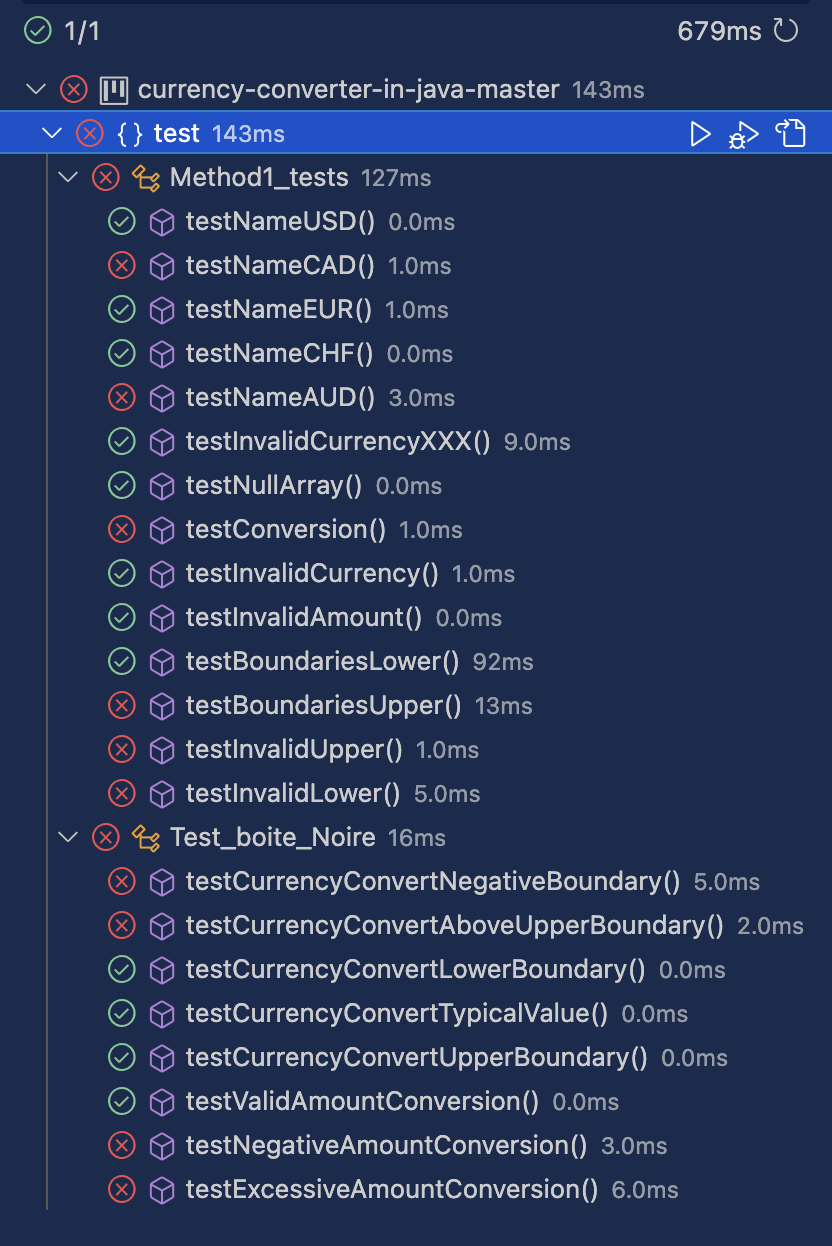
\includegraphics[width=0.32\textwidth]{tests.png}
    \caption{Exécution des tests}
    \end{figure}

\section*{2. Tests Boîte Blanche}
\subsection*{Méthode \texttt{currencyConverter.MainWindow.convert}}   
\begin{itemize}
\item \textbf{Critère de couverture des instructions :}
        \begin{itemize}
          \item D1: {(currency1,currency2,currencies,amount) | currencies.get(i).getName() ==(currency2)}
         \item D2: {(currency1,currency2,currencies,amount) | currencies.get(i).getName() == currency1}
        
    \item \textbf{Jeu de test :}
      
            \item T={("USD","EUR",liste de devises incluant USD et EUR,100.0)}\\
        \end{itemize}

\item \textbf{Critère de couverture des arcs du graphe de flot de contrôle}

\begin{center}
\begin{tikzpicture}[scale=0.13]
\tikzstyle{every node}+=[inner sep=0pt]
\draw [black] (34.7,-4.6) circle (3);
\draw (34.7,-4.6) node {$1$};
\draw [black] (34.7,-13.2) circle (3);
\draw (34.7,-13.2) node {$2$};
\draw [black] (34.7,-22) circle (3);
\draw (34.7,-22) node {$3$};
\draw [black] (34.7,-30.1) circle (3);
\draw (34.7,-30.1) node {$4$};
\draw [black] (34.6,-38.9) circle (3);
\draw (34.6,-38.9) node {$5$};
\draw [black] (34.6,-47.4) circle (3);
\draw (34.6,-47.4) node {$6$};
\draw [black] (34.6,-56.1) circle (3);
\draw (34.6,-56.1) node {$7$};
\draw [black] (61,-4.6) circle (3);
\draw (61,-4.6) node {$8$};
\draw [black] (61,-13.2) circle (3);
\draw (61,-13.2) node {$9$};
\draw [black] (61,-20.4) circle (3);
\draw (61,-20.4) node {$10$};
\draw [black] (61,-28.8) circle (3);
\draw (61,-28.8) node {$11$};
\draw [black] (61,-36.3) circle (3);
\draw (61,-36.3) node {$12$};
\draw [black] (61,-45.1) circle (3);
\draw (61,-45.1) node {$13$};
\draw [black] (61,-54.7) circle (3);
\draw (61,-54.7) node {$14$};
\draw [black] (69,-56.1) circle (3);
\draw (69,-56.1) node {$15$};
\draw [black] (34.7,-7.6) -- (34.7,-10.2);
\fill [black] (34.7,-10.2) -- (35.2,-9.4) -- (34.2,-9.4);
\draw [black] (34.7,-16.2) -- (34.7,-19);
\fill [black] (34.7,-19) -- (35.2,-18.2) -- (34.2,-18.2);
\draw [black] (34.7,-25) -- (34.7,-27.1);
\fill [black] (34.7,-27.1) -- (35.2,-26.3) -- (34.2,-26.3);
\draw [black] (34.6,-41.9) -- (34.6,-44.4);
\fill [black] (34.6,-44.4) -- (35.1,-43.6) -- (34.1,-43.6);
\draw [black] (34.6,-50.4) -- (34.6,-53.1);
\fill [black] (34.6,-53.1) -- (35.1,-52.3) -- (34.1,-52.3);
\draw [black] (37.599,-29.522) arc (84.20322:-85.50534:5.032);
\fill [black] (37.6,-29.52) -- (38.34,-30.1) -- (38.45,-29.11);
\draw [black] (34.67,-33.1) -- (34.63,-35.9);
\fill [black] (34.63,-35.9) -- (35.14,-35.11) -- (34.14,-35.09);
\draw [black] (35.97,-53.43) -- (59.63,-7.27);
\fill [black] (59.63,-7.27) -- (58.82,-7.75) -- (59.71,-8.21);
\draw [black] (61,-7.6) -- (61,-10.2);
\fill [black] (61,-10.2) -- (61.5,-9.4) -- (60.5,-9.4);
\draw [black] (61,-16.2) -- (61,-17.4);
\fill [black] (61,-17.4) -- (61.5,-16.6) -- (60.5,-16.6);
\draw [black] (61,-23.4) -- (61,-25.8);
\fill [black] (61,-25.8) -- (61.5,-25) -- (60.5,-25);
\draw [black] (61,-31.8) -- (61,-33.3);
\fill [black] (61,-33.3) -- (61.5,-32.5) -- (60.5,-32.5);
\draw [black] (61,-39.3) -- (61,-42.1);
\fill [black] (61,-42.1) -- (61.5,-41.3) -- (60.5,-41.3);
\draw [black] (61,-48.1) -- (61,-51.7);
\fill [black] (61,-51.7) -- (61.5,-50.9) -- (60.5,-50.9);
\draw [black] (63.96,-55.22) -- (66.04,-55.58);
\fill [black] (66.04,-55.58) -- (65.34,-54.95) -- (65.17,-55.94);
\draw [black] (63.679,-5.947) arc (60.52529:-42.8658:30.987);
\fill [black] (71.14,-54) -- (72.05,-53.76) -- (71.32,-53.08);
\draw [black] (63.609,-14.678) arc (57.32813:-36.20173:27.299);
\fill [black] (70.9,-53.78) -- (71.78,-53.43) -- (70.97,-52.84);
\draw [black] (58.483,-18.929) arc (-144.02902:-215.97098:3.624);
\fill [black] (58.48,-14.67) -- (57.61,-15.03) -- (58.42,-15.61);
\draw [black] (36.85,-28.01) -- (58.85,-6.69);
\fill [black] (58.85,-6.69) -- (57.92,-6.89) -- (58.62,-7.6);
\end{tikzpicture}
\end{center}

\item\textbf{Critère de couverture des chemins indépendants du graphe de flot de contrôle}
\begin{itemize}
    \item 1 2 3 4 5 6 7 8 9 10 11 12 13 14 15
    \item T={("USD", "EUR", liste de devises incluant USD et EUR, 100.0)}
\end{itemize}

\item \textbf{Critère de couverture des conditions}\\
Non-applicable.\\ On n'a pas de conditions composées.

\item \textbf{Critère de couverture des i chemins}
 \begin{itemize}
    \item \textbf{Jeu de test :}
      
            \item On saute boucle : currencies est vide
            \item 1 iteration - on veut un currencies de taille 1: T={("USD","EUR",liste de devises avec uniquement USD,100.0)}
            \item 2 iterations - on veut un currencies de taille 1: T={("USD","EUR",liste de devises avec uniquement USD et EUR,100.0)}
            \item m iterations - on veut un currencies de taille m: T={("USD","EUR",liste de devises avec m donnees,100.0)}
            
        \end{itemize}
\end{itemize}

\subsection*{Méthode currencyConverter.Currency.convert(Double, Double)}
\begin{itemize}
   \item \textbf{Critère de couverture des instructions :}
        \begin{itemize}
          \item D1: {(price = amount * exchangeValue)}
         \item D2: {(price = Math.round(price * 100d) / 100d)}
        
    \item \textbf{Jeu de test :}
      
            \item T={("USD","EUR","GBP","CHF","CNY","JPY",Montant au-delà et entre de l'intervalle [0,1000000])}\\
        \end{itemize}
   
    \item \textbf{Critère de couverture des arcs du graphe de flot de contrôle:}
        \begin{itemize}
            \item Ce critère n'est pas applicable car il n'y a pas d'instructions conditionnelles (branches if-else) dans la méthode Currency.convert.
        \end{itemize}    
        
    \item \textbf{Critère de couverture des chemins indépendants du graphe de flot de contrôle:}
    \begin{itemize}
        \item Semblable à la couverture des branches, ce critère n’est pas non plus applicable en raison de l’absence de chemins conditionnels. Il n’existe qu’un seul chemin d’exécution dans la méthode.
    \end{itemize}
    
    \item \textbf{Critère de couverture des conditions:}
    \begin{itemize}
        \item Étant donné qu'aucune condition booléenne n'est évaluée dans la méthode, ce critère ne s'applique pas à la méthode Currency.convert
    \end{itemize}
    
    \item \textbf{Critère de couverture des i-chemins:}
    \begin{itemize}
        \item Il n'y a pas de boucles dans la méthode Currency.convert, ce critère ne peut donc pas être appliqué.
    \end{itemize}
    
\end{itemize}


\section*{Résultats des tests et observations}
Suite aux tests de la méthode MainWindow.convert. Nous nous sommes aperçus de plusieurs soucis. En effet, nos tests ne passaient pas. Ceci était dû à une comparaison de Currency Name au lieu de Currency Short Name comme le voulait la spécification. De plus, certaines monnaies mentionnées dans la spécification ne figurait pas dans la méthode init(). Finalement, == ne devrait pas être utilisé avec des String. .equals() aurait été plus approprié.\\\\





\end{document}
